\documentclass[a4paper,11pt,french]{article}
\usepackage[utf8]{inputenc}

\usepackage[T1]{fontenc}
\usepackage[francais]{babel}
\usepackage[top=1.5cm, bottom=2cm, left=1.5cm, right=1.5cm, includeheadfoot]{geometry} %pour les marges
\usepackage{lmodern}
\usepackage{tikz}        
\usepackage{fancyhdr} % Required for custom headers
\usepackage{lastpage} % Required to determine the last page for the footer
\usepackage{extramarks} % Required for headers and footers
\usepackage{graphicx} % Required to insert images
\usepackage{tabularx, longtable}
\usepackage{color, colortbl}
\usepackage{amsmath}
\usepackage{mathtools}
\usepackage{amssymb}
\usepackage[toc,page]{appendix} 
\usepackage{pgfplots}
\usepackage{eurosym}
\usepackage{rotating}
\usepackage{array}
\usepackage{cmbright}
\usepackage[hidelinks]{hyperref}
\usepackage[french]{algorithm2e}
\usepackage{cmbright}
\usepgflibrary{arrows} % for pgf-umlsd

\linespread{1.1} % Line spacing


\setlength{\headheight}{40pt}
\linespread{1.1} % Line spacing

% Set up the header and footer
\pagestyle{fancy}
\lhead{\textbf{\hmwkClass -- \hmwkSubject \\ \hmwkTitle \\ \hmwkDocName}} % Top left header
\rhead{
\includegraphics[width=10em]{logo_univ.png}}
\lfoot{\lastxmark} % Bottom left footer
\cfoot{} % Bottom center footer
\rfoot{Page\ \thepage\ / \pageref{LastPage}} % Bottom right footer
\renewcommand\headrulewidth{0.4pt} % Size of the header rule
\renewcommand\footrulewidth{0.4pt} % Size of the footer rule

\setlength{\headheight}{40pt}

\newcommand{\hmwkTitle}{Audit des implantations SSL/TLS} % Assignment title
\newcommand{\hmwkClass}{Master 2 SSI } % Course/class
\newcommand{\hmwkAuthorName}{Claire Smets, William Boisseleau,\\ &&Pascal Edouard, Mathieu Latimier,\\ &&Julien Legras} % Your name
\newcommand{\hmwkSubject}{Conduite de projet} % Subject
\newcommand{\hmwkDocName}{Rapport préliminaire -- Audit de clefs cryptographiques} % Document name

\newcommand{\version}{1.2} % Document version
\newcommand{\docDate}{5 février 2014} % Document date
\newcommand{\checked}{} % Checker name
\newcommand{\approved}{Ayoub Otmani} % Approver name

\definecolor{gris}{rgb}{0.95, 0.95, 0.95}

\begin{document}
\pagestyle{fancy}

\vspace*{5cm}
\begin{center}\textbf{\Huge{\hmwkDocName}}\end{center}
\vspace*{7cm}
	
\begin{center}
\fcolorbox{black}{gris}{
\begin{minipage}{10cm}
\begin{tabularx}{10cm}{lXl}
	\bfseries{Date} & & \docDate\\
	& & \\
	\bfseries{Rédigé par} & & \hmwkAuthorName \\
	& & \\
	\bfseries{À l'attention de} & & \approved \\
	& & \\
\end{tabularx}
\end{minipage}
}
\end{center}


\pagebreak

\section{Introduction}
Cette première partie du projet consiste à faire une étude des clefs cryptographiques RSA circulant sur Internet.
Nous avons donc dans un premier temps récupéré une liste d'adresses IP dont le port 443 (HTTPS) était ouvert.

Ensuite, nous avons tenté de récupérer les certificats de toutes les adresses listées. Cette récupération s'occupait également d'extraire les moduli et les clefs publiques des certificats, mais aussi de stocker une liste de certificats doublons.

Enfin, avec tous les moduli que nous avons extraits, nous avons pu construire deux arbres permettant de définir si des moduli contiennent des facteurs premiers communs.

\section{ZMAP}

ZMAP est un outil permettant de faire des scans réseau. 
Il est capable de scanner toutes les adresses IPv4 possibles, avec une moyenne de 1.4 millions de paquets envoyés par secondes sur les connexions à très haut débit.

Nous l'avons utilisé pour scanner l'ensemble des adresses IPv4, en envoyant simplement des paquets SYN aux adresses visées sur le port 443 pour SSL.

Pour l'installer sur nos machines, voici la procédure à suivre :

\begin{enumerate}
\item Installation des dépendances :
\begin{verbatim}
~ $ sudo apt-get install cmake libgmp3-dev libpcap-dev gengetopt byacc flex git
\end{verbatim}
\item Récupération des sources de ZMap :
\begin{verbatim}
~ $ git clone git://github.com/zmap/zmap.git
\end{verbatim}
\item Compilation :
\begin{verbatim}
~ $ cd zmap
~/zmap $ mkdir build
~/zmap $ cd build
~/zmap/build $ cmake .. -DENABLE_HARDENING=ON
~/zmap/build $ make
~/zmap/build $sudo make install
\end{verbatim}
\end{enumerate}

Il y a plusieurs options disponibles, nous avons utilisé la commande suivante pour effectuer notre scan :
\begin{verbatim}
# zmap -p 443 -o scan_output_zmap
\end{verbatim}

\section{Application RC}

Une fois que l'on avait la liste fournie par ZMAP, il nous restait à récupérer les certificats sur les serveurs dont le port SSL était ouvert, en établissant une connexion sur chacun d'eux.

Pour cela nous avons codé deux scripts perl, l'un pour la récupération de certificat SSH (que nous n'avons pas testé à cause de l'avertissement reçu), et un autre pour la récupération de certificats SSL (ssl\_collector.pl).

Commandes OpenSSL utilisées :
\begin{itemize}
\item pour l'établissement de la connexion (avec s\_client) :

\begin{verbatim}
echo  \" \" | timeout 20 openssl s_client -connect $addr:443 -sess_out tmp_$addr.pem 
-ignore_critical -showcerts -CApath /etc/ssl/certs > /dev/null 2> tmp_$addr.log
\end{verbatim}
\item  pour la capture de session (avec sess\_id) :
\begin{verbatim}
openssl sess_id -in tmp_$addr.pem -cert > certs/$addr.pem 2> tmp_$addr.log
\end{verbatim}
\item pour la récupération du certificat et de la clé privée :
\begin{verbatim}
openssl x509 -in certs/$addr.pem -noout -pubkey > keys/$addr.pem 2> tmp_$addr.log
\end{verbatim}
\end{itemize}

Pour ce qui est de la gestion des doublons, nous avons également créé un autre script perl (clean.pl).

La chaîne d'utilisation est donc la suivante :
\begin{verbatim}
~ $ ./ssl_collector ips.txt
~ $ ./clean.pl
\end{verbatim}

\section{Factorisation}

L'objectif final de cette première partie était de déterminer s'il existait des facteurs premiers communs
parmi les clefs récupérées. Pour cela nous avons développé deux arbres de factorisation.
Lors du scan nous avions récupéré 85.000 certificats uniques, mais nous avons également souhaité faire la factorisation avec les données du projet Sonar de Rapid7 Labs avec 523 000 certificats.

Le premier arbre se contente de multiplier l'ensemble des moduli par groupe de deux.
Le second arbre calcule deux modulos du résultat produit, selon le carré des résulats stockés par l'arbre des produits (aux étapes intermédiaires) :

Une fois le second arbre calculé, les dernières feuilles des arbres indiquent soit un PGCD(res\_final, N$_i$ ) = 1 (donc avec des entiers premiers uniques), ou un PGCD(res\_final, N$_i$ ) = p (entier premier non unique).

Voici les algorithmes de ces deux arbres :

\begin{algorithm}[H]
\label{alg:productTree}
 %\SetAlgoLined % For previous releases [?]
 \Entree{Tableau des moduli des clefs publiques : T}
 \Sortie{Hauteur de l'arbre, produits des moduli des clefs publiques}
 \Donnees{Tableaux v, tmp; Entier i, level}
 $v \leftarrow T$\;
 $level \leftarrow 0$\;
 \Tq{$|v|>1$}{
  $tmp \leftarrow \emptyset$\;
  \PourCh{$i \in \{0, .., |v| / 2\}$}{
    $tmp[i] \leftarrow v[i\times2] \times v[i\times2 + 1]$\;
  }
  $storeProductLevel(v, level)$\;
  $v \leftarrow tmp$\;
  $level \leftarrow level + 1$\;
 }
 \Retour{level}
 \caption{Construction de l'arbre des produits}
 
\end{algorithm}
\vspace{1cm}
\begin{algorithm}[H]
 \label{alg:remainderTree}
 %\SetAlgoLined % For previous releases [?]
 \Entree{Hauteur de l'arbre des produits : level}
 \Sortie{PGCDs des moduli des clefs publiques}
 \Donnees{Tableaux P, v, w; Entier i}
 $P \leftarrow getProductLevel(level)$\;
 \Tq{$level>0$}{
  $v \leftarrow getProductLevel(level - 1)$\;
  \PourCh{$i \in \{0, .., |v|\}$}{
    $v[i] \leftarrow P[i/2] \pmod{v[i]^2}$\;
  }
  $level \leftarrow 1$\;
  $storeRemainderLevel(v, level)$\;
  $v \leftarrow tmp$\;
  $level \leftarrow level + 1$\;
 }
 $w \leftarrow \emptyset$\;
 \PourCh{$i \in \{0, .., |v|\}$}{
    $w[i] \leftarrow P[i/2] \pmod{v[i]^2}$\;
    $w[i] \leftarrow w[i] / v[i]$\;
    $w[i] \leftarrow pgcd(w[i],v[i])$\;
  }
 \Retour{w}
 \caption{Construction de l'arbre des restes}
\end{algorithm}


Lors de nos tâches d'optimisation, nous avons réalisé qu'il était possible de construire l'arbre entier (product tree + remainder tree), en mémoire vive (nous avons donc créé une option fullRAM à notre algo).

L'algorithme est le même, seul le choix de la structure change.
Dans la première méthode, nous utilisions des fichiers binaires GMP à chaque étape de construction, dans la  seconde nous stockons l'intégralité de l'arbre des produits en mémoire.

Pour accélérer la construction de l'arbre, nous utilisons des \textit{threads}, qui parallélisent le traitement de chaque niveau d'arbre (sur la largeur de l'arbre).
Nous avons tenté d'améliorer encore le procédé, en parallélisant le calcul sur la hauteur de l'arbre. Il s'est avéré que ce n'était pas aussi efficace, nous avons donc abandonné cette partie.

Pour compiler le programme :
\begin{verbatim}
~ $ sudo apt-get install libgmp-dev cmake git 
~ $ git clone https://github.com/RandomGuys/fact.git
~ $ cd fact
~/fact $ mkdir build
~/fact $ cd build
~/fact/build $ cmake ..
~/fact/build $ make
~/fact/build $ sudo make install
\end{verbatim}

Il y a également un \textit{man} qui s'installe, vous pouvez donc consutler l'aide avec la commande \verb+man fact+.

Pour utiliser ce programme, la ligne de commande est la suivante :
\begin{verbatim}
$ fact -m mes_moduli --fullram|--files [--format hexa|decimal]
\end{verbatim}


\section{Conclusion des résultats produits}

\subsection{Fichier de résultats}
Les résultats se trouvent dans le fichier \verb+moduli_p_q+ construit de la façon suivante :
\begin{verbatim}
modulus, facteur commun, facteur déduit
...
\end{verbatim}
\subsection{Premiers chiffres}
Voici les premiers chiffres obtenus des scans :
\begin{center}
\begin{tabular}{|r|c|c|}
\hline
\textbf{}&\textbf{Scan 1}&\textbf{Scan Sonar}\\
\hline
\textbf{moduli}&85 636&523 017\\
\hline
\textbf{vulnérables}&104 (0,12\%)&2 382 (0,46\%)\\
\hline
\textbf{facteurs communs}&11&757\\
\hline
\textbf{autres facteurs}&104&2 382\\
\hline
\textbf{total facteurs}&115&3 139\\
\hline
\end{tabular}
\end{center}

En comparant avec les résultats du projet factorable de l'Université de Californie et de l'Université du Michigan, nous obtenons un pourcentage de clefs vulnérables assez proche. En effet, ils ont obtenu 0,50\% de clefs vulnérables et nous en avons trouvées 0,46\% 

Pour la suite de l'analyse des résultats, nous nous sommes focalisés sur le scan Sonar.

\subsection{Entropie}
Le graphe suivant représente le pourcentage d'entropie des 757 facteurs premiers trouvés. Ce niveau d'entropie a été calculé selon l'entropie de Shannon (représentation binaire des clefs). Nous nous sommes basés sur la bibliothèque \verb+libdisorder+ (\url{http://libdisorder.freshdefense.net/}) qui fournit un programme de tests. Ce dernier a été modifié pour nos besoins et pour pouvoir injecter les résultats dans gnuplot pour obtenir le graphe suivant :

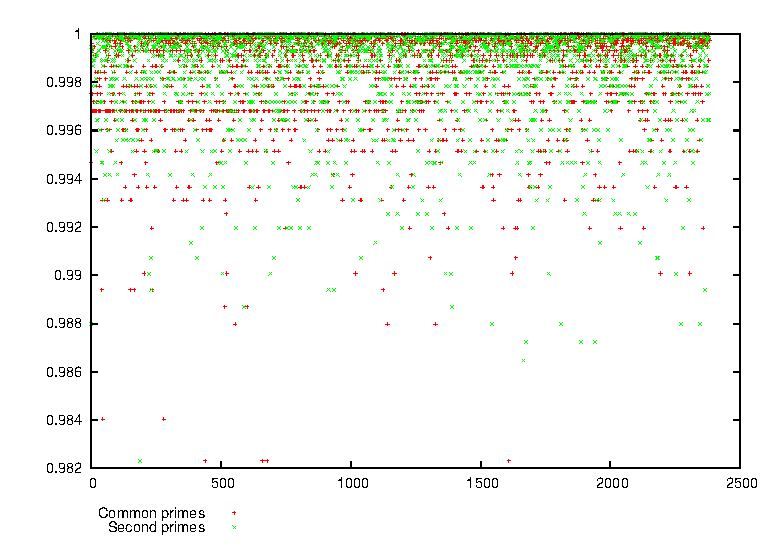
\includegraphics[width=16cm]{entropyprimes.eps}
\\
Entropie moyenne des facteurs communs : 0.998518\\
Entropie moyenne des second facteurs : 0.998551\\

\subsection{Tailles des clefs}
Dans nos résultats, nous pouvons constater que seules deux tailles de clefs apparaissent : 512 et 1024 bits. Voici les chiffres :

\begin{center}
\begin{tabular}{|r|c|c|}
\hline
\textbf{}&\textbf{512 bits}&\textbf{1024 bits}\\
\hline
\textbf{Total}&2 345&318 558\\
\hline
\textbf{Vulnérables}&6 (0,26\%)&2 376 (0,75\%)\\
\hline
\end{tabular}
\end{center}

Nous avions également d'autres tailles de clefs en entrée mais leur nombre devait être trop petit par rapport à l'espace des clefs de cette taille pour obtenir des facteurs communs.

\end{document}
